%!TEX root = ../Main.tex
\section{Processes}
\label{s:Processes}

Each combinator defines a stream process which is expressed in terms of a simple imperative program with a local heap.
The process pulls data from an arbitrary number of input streams and pushes data to at least one output stream.
Each input array is converted to its own process with a single output stream, which repeatedly pushes the values from the array.
% \ben{Mention how we're going to convert arrays to streams, but we don't need to give the details yet}. 

% make it explicit that the processes are only an intermediate repr
The process language is used for the implementation of combinators and as an intermediate representation for fusion, while the original program using these combinators can be written without any knowledge of processes.


% -----------------------------------------------------------------------------
\subsection{Grouping}
\begin{figure}

\begin{center}
\begin{alltt}
           group 
             = \(\lambda\) (s1: Stream Nat) (s2: Stream Nat). 
               \(\nu\) (f: Bool) (l: Nat) (v: Nat) (A0..A3: Label).
\end{alltt}
\begin{code}
               process
               { ins:    { s1 }
               , outs:   { s2 }
               , heap:   { f = T, l = 0, v = 0 }
               , label:  A0
               , instrs: { A0 = pull s1 v            A1 {}
                         , A1 = case (f || (l /= v)) A2 {}  A3 {}
                         , A2 = push s2 v            A3 { l = v, f = F }
                         , A3 = drop s1              A0 {} } }
\end{code}
\end{center}
\vspace{1em}
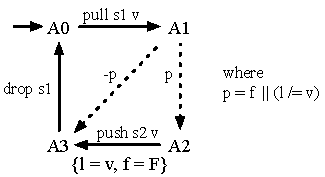
\includegraphics[scale=1.1]{figures/state-group.pdf}
\caption{The group combinator}
\label{fig:Process:Group}
\end{figure}

The definition of the @group@ combinator which removes consecutive elements from its input stream is given in Fig.~\ref{fig:Process:Group}. We include the concrete code representation as well as a diagram of the state machine defined by the associated stream process.

The @group@ combinator has two parameters, @s1@ and @s2@, which bind the input and output streams respectively. The \emph{nu-binders} \mbox{$\nu$ @(f: Bool) (l: Nat)@...} indicate that each time the @group@ combinator is instantiated, fresh names must be given to @f@, @l@ and so on, that do not conflict with other instantiations. 

The body of the combinator is a record that defines the process. The @ins@ field of the record defines the set of input streams and the @outs@ field the set of output streams. The @heap@ field gives the initial values of each of the local variables. The @instrs@ field contains a set of labeled instructions that define the program, while the @label@ field gives the label of the initial instruction. 

The initial instruction @(pull s1 v A1 {})@ pulls the next element from the stream @s1@, writes it into the heap variable @v@ (value), then proceeds to the instruction at label @A1@.
The empty set @{}@ after the target label @A1@ can be used to update values in the heap, but as we do not need to perform heap updates here we leave it empty. 

Next, the instruction @(case (f || (l /= v)) A2 {} A3 {})@ checks whether the predicate @(f || (l /= v))@ is true; if so it proceeds to the instruction at label @A2@, otherwise it proceeds to the instruction at label @A3@.
We use the variable @l@ (last) to track the last value read from the stream, and the boolean @f@ (first) to track whether this is the first element.

When the above predicate is true, the instruction @(push s2 v A3 { l = v, f = F })@ pushes the value @v@ to the stream @s2@ and proceeds to the instruction at label @A3@, once the heap has been updated to set variable @l@ to @v@ and @f@ to @F@ (False). 

Finally, the instruction @(drop s1 A0 {})@ signals that the current element that was pulled from stream @s1@ is no longer required, and goes back to the first the instruction at @A0@.
This @drop@ instruction is used to coordinate processes when performing fusion and concurrent evaluation; the next element of a stream may only be pulled after all consuming processes have pulled and dropped the current element.
% This @drop@ instruction is a synchronisation primitive that is used in the fusion algorithm and concurrent evaluation, but has no direct operational meaning.
% We discuss @drop@ further in \TODO{ref}. 

Overall, the @f@ variable tracks whether we are dealing with the first value from the stream, @l@ holds the last value pulled from the stream (or 0 if none have been read yet), and @v@ holds the current value pulled from the stream.
The process emits the first value pulled from the stream and every value that is different from the last one that was pulled.
For example, when executed on the input stream $[1, 2, 2, 3]$, this process will produce the output $[1, 2, 3]$.

Note that we refer to @group@ itself as a \emph{combinator} as it is parameterised by the names of the streams it deals with (@s1@ and @s2@). Once the combinator has been instantiated to work on particular streams the result is a concrete \emph{process}, which is the code representation of a state machine.


% Recall that @group@ removes consecutive duplicates from its input stream.
% It has one input, @file1@, and one output, @uniques@.

% There are three variables in the heap: @first@ is initialised to @True@ as the first pulled value has no last value to compare against; @value@ stores the most recently pulled value, and @last@ stores the last pulled value.

% The @last@ and @value@ variables are initialised to $0$, but could be initialised to any value: these initial values will not be used.
% The initial label is @L0@, which pulls from the input @file1@. This blocks waiting for an input value, and when one is received, it is stored in @value@ and the process moves to @L1@.
% Instruction @L1@ performs a case analysis on a boolean: if it is the first read value, or the last value is not equal to the most recent value, it jumps to @L2@; otherwise it jumps to @L3@.
% Instruction @L2@ pushes the most recent value to the output and jumps to @L3@, updating the last value to the most recent value, and setting first to @False@.
% Finally, the instruction for @L3@ `drops' the recently pulled value from @file1@ and jumps back to @L0@.
% This dropping is required to coordinate between multiple processes that read from the same input: now that the read value from @file1@ has been dropped, another process is free to pull the next value from @file1@ if it so wishes.



% -----------------------------------------------------------------------------
\subsection{Merging}
\begin{figure}
\begin{alltt}
               merge
                 = \(\lambda\) (s1: Stream Nat) (s2: Stream Nat) (s3: Stream Nat). 
                   \(\nu\) (x1: Nat) (x2: Nat) (B0..E2: Label).
\end{alltt}
\begin{code}
                   process
                   { ins:    { s1, s2 }
                   , outs:   { s3 }
                   , heap:   { x1 = 0, x2 = 0 }
                   , label:  B0
                   , instrs: { B0 = pull s1 x1     B1 {}
                             , B1 = pull s2 x2     C0 {}
                             , C0 = case (x1 < x2) D0 {}  E0 {}
                             , D0 = push s3 x1     D1 {}
                             , D1 = drop s1        D2 {}
                             , D2 = pull s1 x1     C0 {}
                             , E0 = push s3 x2     E1 {}
                             , E1 = drop s2        E2 {}
                             , E2 = pull s2 x2     C0 {} } }
\end{code}

\medskip
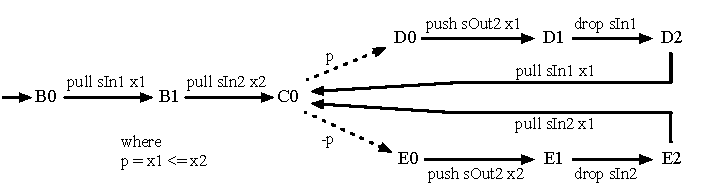
\includegraphics[scale=1.1]{figures/state-merge.pdf}
\caption{The merge combinator}
\label{fig:Process:Merge}
\end{figure}

The definition of the @merge@ combinator, which merges two input streams, is given in Fig.~\ref{fig:Process:Merge}.
The combinator binds the two input streams to @s1@ and @s2@, while the output stream is @s3@.
The two heap variables @x1@ and @x2@ are used to store the currently read values from each input.
The process starts by pulling from both input streams, then compares the two values, and pushes the smaller of the values to the output stream.
It then drops the input stream corresponding to the smaller value, then pulls from the same stream, and performs the same comparison again.
% The forms of the instructions used to define this combinator are the same as the @group@ combinator in the previous section.
% We only need the four basic @pull@, @case@, @push@ and @drop@ instructions.

As this process merges infinite streams, if we execute it with a finite input prefix, the result will be an intermediate state that may not yet have pushed all available output.
For example, if we execute the process with the input streams $[1, 4]$ and $[2, 3, 100]$ then the values $[1, 2, 3, 4]$ will be pushed to the output.
After pushing the last $4$, the process will block at instruction @E2@, waiting for the next value to be pulled from @s2@.
We discuss how to handle finite streams later in ~\S\ref{s:Finite}.


% The instructions at @L0@ and @L1@ initialise the process by reading the first values from each stream, then move to @C0@.
% Instruction @C0@ checks which value is smaller: if the value @a@ read from @file1@ is smaller, it moves to @A0@; otherwise it moves to @B0@.
% Instructions @A0@, @A1@ and @A2@ push @file1@'s value to the output, drop it, and pull another one before moving back to @C0@ to compare again.
% Instructions @B0@, @B1@ and @B2@ are equivalent, except performing on @file2@ instead.


% -----------------------------------------------------------------------------
\clearpage{}
\subsection{Fusion}
Our fusion algorithm takes two process state machines and produces a new one that computes the outputs of both.
For example, suppose we need to produce a single machine that computes the outputs of the first two combinators of our @uniquesUnion@ example back in \S\ref{s:Introduction}.
We want a result machine that computes both a @group@ machine and a @merge@ machine executed in parallel, where the first input stream of the @merge@ is the same as the input stream of the @group@.
Compared to the @uniquesUnion@ example, we will associate a stream named @s1@ with the first array (@arr1@) and a stream named @s2@ with the second array (@arr2@). 


% -----------------------------------------------------------------------------
\subsubsection{Fusing Pulls}
\begin{figure}
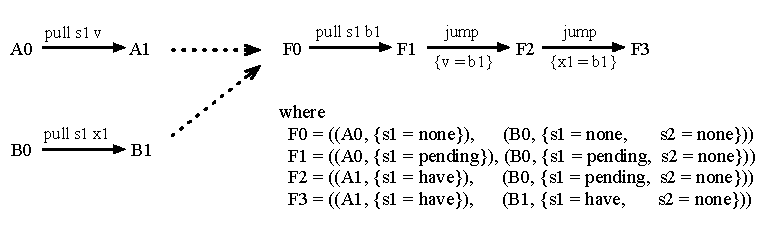
\includegraphics[scale=1.1]{figures/fuse-pull-pull.pdf}
\caption{Fusing pull instructions}
\label{fig:Fusion:Pulls}
\end{figure}

The algorithm proceeds by considering pairs of states: one in each of the machines to be fused.
Both the @group@ machine and the @merge@ machine pull from the same stream as their initial instruction, so we have the situation shown in Fig.~\ref{fig:Fusion:Pulls}.
The @group@ machine needs to transition from label @A0@ to label @A1@, and the @merge@ machine from @B0@ to @B1@.
In the result machine we produce three new instructions that transition between four result states, @F0@ to @F3@.
Each of the result states represents a combination of two original states, one from each of the input machines.
For example, the first result state @F0@ represents a combination of the @group@ machine being in its initial state @A0@ and the @merge@ machine being in its own initial state @B0@. 

We also associate each of the result states with information describing whether or not each machine has already pulled a value from each input stream, which is used to determine whether another value can be pulled.
For the @F0@ case shown in Fig.~\ref{fig:Fusion:Pulls} we have ((A0, \{s1 = none\}), (B0, \{s1 = none, s2 = none\})).
This means that the result state @F0@ represents a combination of the two input states @A0@ and @B0@.
As both @A0@ and @B0@ are the initial states of their respective machines, those machines have not yet pulled any values from their two input streams, so both @s1@ and @s2@ are set to `none'.

From the joint state @F0@, both of the input machines need to pull from stream @s1@, the @group@ machine storing the value in a variable @v@ and the @merge@ machine storing it in @x1@.
In the result machine this is managed by storing the pulled value in a fresh buffer variable @b1@, and then using later instructions to copy the value into the original variables @v@ and @x1@.
For this we use the @jump@ instruction which transitions between states without affecting any of the input or output streams.
After the algorithm has completed fusing both processes it may be possible to eliminate redundant @jump@, depending on how the affected variables are used by other instructions.

Finally, note that in the result states @F0@ through @F3@ the state of the input streams transitions from `none', to `pending' then to `have'.
The `none' state means that we have not yet pulled a value from the associated stream.
The `pending' state means we have pulled a value into the stream buffer variable (@b1@ in this case).
The `have' state means that we have copied the pulled value from the stream buffer variable into the local variable used by each machine.
In Fig.~\ref{fig:Fusion:Pulls},  `s1' is set to `have' in @F2@ after we have set `v = b1', while `s1' is set to `have' in @F3@ after we have set `x1 = b1'. 


\eject{}
% -----------------------------------------------------------------------------
\subsubsection{Fusing Cases}
\begin{figure}
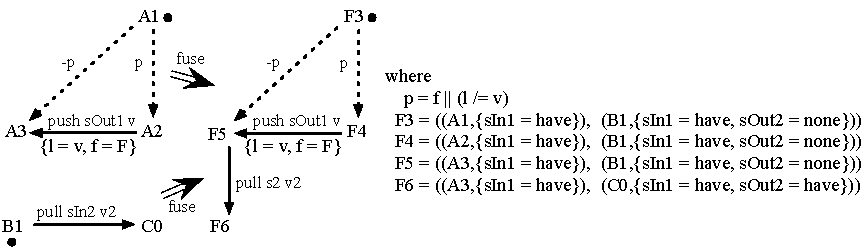
\includegraphics[scale=1.1]{figures/fuse-case-pull.pdf}
\caption{Fusing case instructions}
\label{fig:Fusion:Case}
\end{figure}

Once the result machine has arrived in the joint state @F3@, this is equivalent to the two input machines arriving in states @A1@ and @B1@ respectively.
Fig.~\ref{fig:Fusion:Case} shows the next few transitions of these machines.
From state @A1@, the @group@ machine needs to perform a @case@ branch to determine whether to push the current value it has from its input stream @s1@ to its output stream, which we name @s3@ --- or to just move on to the next value from its input.
From state @B1@, the @merge@ machine needs to pull a value from its second input stream @s2@. 

In the fused result, @F3@ performs the case analysis from @A1@, moving to either @A2@ or @A3@, corresponding to @F4@ and @F5@ respectively.
At @F4@, the push at @A2@ is executed and moves to @A3@, corresponding to @F5@.

Finally, at @F5@ the @merge@ machine pulls from @s2@, moving from @B1@ to @C0@.
Because the stream @s2@ is only pulled from by the @merge@ machine, no coordination is required between @merge@ and @group@ for this pull.
In this case, we simply perform a @pull@ instruction.

In terms of fusion, we could construct the result machine in multiple ways.
One option is to perform the case branch first and then pull from @s2@.
We could alternately pull from @s2@ first and then perform the case branch.
By construction, the predicate used in the branch only refers to variables local to the @group@ machine, and the pull instruction from @B1@ stores its result in a variable local to the @merge@ machine.
As the set of variables does not overlap, either ordering is correct.
For this example we choose to perform the branch first, though will discuss the ramifications of this choice further in \S\ref{s:FusionOrder}.

% -----------------------------------------------------------------------------
\subsection{Fused Result}

Fig.~\ref{fig:Process:Fused} shows the result of fusing @group@ and @merge@ together.
The process has two inputs, @s1@ and @s2@, which correspond to the original input streams.
Of the two outputs, @s3@ is the @group@'s output stream, while @s4@ is the @merge@'s output stream.
The heap contains the variables from both processes, as well as the new buffer variable @b1@, which has been initialised to $0$.

\TODO{More explanation}

\begin{figure}
\begin{code}
            process
            { ins:    { s1, s2 }
            , outs:   { s3, s4 }
            , heap:   { f = T, l = 0, v = 0, x1 = 0, x2 = 0, b1 = 0}
            , label:  F0
            , instrs:

  (shared pull)
              { F0  = pull s1 b1            F1  {}

  (merge label B0)
              , F1  = jump                  F2  {v  = b1}

  (group labels A0-A3)
              , F2  = jump                  F3  {x1 = b1}
              , F3  = case (f || (l /= v))  F4  {}                F5  {}
              , F4  = push s3 v             F5  {l  = v, f  = F}
              , F5  = jump                  F6  {}

  (merge label B1)
              , F6  = pull s2 x2            F7  {}

  (merge label C0)
              , F7  = case (x1 < x2)        F8  {}                F16 {}

  (merge labels D0-D1)
              , F8  = push s4 x1            F9  {}
              , F9  = drop s1               F10 {}

  (shared pull)
              , F10 = pull s1 b1            F11 {}

  (group labels A0-A3)
              , F11 = jump                  F12 {v  = b1}
              , F12 = case (f || (l /= v))  F13 {}                F14 {}
              , F13 = push s3 v             F14 {l  = v, f  = F}
              , F14 = jump                  F15 {}

  (merge label D2)
              , F15 = jump                  F7  {x1 = b1}

  (merge labels E0-E2)
              , F16 = push s4 x2            F17 {}
              , F17 = drop s2               F18 {}
              , F18 = pull s2 x2            F7  {} } }
\end{code}

% With original label names and 'n', 'h' and 'p' for input state
%\begin{code}
%A0nB0n = pull s1 b1  A0pB0p{}
%A0pB0p = jump        A1hB0p{v  = b1}
%A1hB0p = jump        A1hB1h{x1 = b1}
%
%A1hB1h = case (f || (l /= v))
%                     A2hB1h{}
%                     A3hB1h{}
%
%A2hB1h = push s3 v   A3hB1h{l  = v, f  = F}
%A3hB1h = jump        A0nB1h{}
%A0nB1h = pull s2 x2  A0nC0h{}
%
%A0nC0h = case (x1 < x2)
%                     A0nD0h{}
%                     A0nE0h{}
%
%A0nD0h = push s4 x1  A0nD1h{}
%A0nD1h = drop s1     A0nD2n{}
%A0nD2n = pull s1 b1  A0pD2p{}
%A0pD2p = jump        A1hD2p{v  = b1}
%
%A1hD2p = case (f || (l /= v))
%                     A2hD2p{}
%                     A3hD2p{}
%
%A2hD2p = push s3 v   A3hD2p{l  = v, f  = F}
%A3hD2p = jump        A0nD2p{}
%A0nD2p = jump        A0nC0h{x1 = b1}
%
%A0nE0h = push s4 x2  A0nE1h{}
%A0nE1h = drop s2     A0nE2h{}
%A0nE2h = pull s2 x2  A0nC0h{}
%\end{code}

% Cleaned up, simplified, variables collated
% \begin{code}
%             process
%             { ins:    { s1, s2 }
%             , outs:   { s3, s4 }
%             , heap:   { f = T, l = 0, x1 = 0, x2 = 0}
%             , label:  F0
%             , instrs: { F0 = pull s1 x1              F3 {}
%                       , F3 = case (f || (l /= x1))   F4 {} F5 {}
%                       , F4 = push s3 x1              F5 { l = x1, f = F }
%                       , F5 = pull s2 x2              F6 {}
% 
%                       , F6 = case (x1 < x2)          A0 {} B0 {}
% 
%                       , A0 = push s4 x1              A1 {}
%                       , A1 = drop s1                 A2 {}
%                       , A2 = pull s1 x1              A3 {}
%                       , A3 = case (f || (l /= x1))   A4 {} F6 {}
%                       , A4 = push s3 x1              F6 { l = x1, f = F }
% 
%                       , B0 = push s4 x2              B1 {}
%                       , B1 = drop s2                 B2 {}
%                       , B2 = pull s2 x2              F6 {} } }
% \end{code}
\caption{Fusion of group and merge}
\label{fig:Process:Fused}
\end{figure}



\clearpage{}
\subsection{Process definitions}

%% This figure is referenced below, in 'Process definitions', but putting it up here before the big fused process stops the fused one from splitting across multiple pages.
%!TEX root = ../Main.tex

\begin{figure}
\begin{minipage}[t]{0.4\textwidth}
\begin{tabbing}
\Instr \TABDEF @MMMM@  \TABSKIP $\Exp$ \TABSKIP $\Exp$ \TABSKIP $\Exp$ \kill

\Exp,~$e$ \> $\to$ \> $x~|~v~|~e~e $ \\
  \> $\enskip|~$ \> $ (e~||~e) ~|~ e+e ~|~ e~@/=@~e ~|~ e < e$ \\
\Value,~$v$ \> $\to$ \> $\mathbb{N}~|~\mathbb{B}~|~(\lambda{}x.~e)$ \\
\Heap,~$\Sigma$ \> $\to$ \> $\cdot~|~\Sigma,~x~=~v$ \\
\\

\Proc \>:=\> @process@ \\
MMMMMM \= M \= \kill
\> \> @ins:   @  $(\Chan ~\mapsto~ \InputState)$ \\
\> \> @outs:  @  $\sgl{\Chan}$ \\
\> \> @heap:  @  \Heap \\
\> \> @label: @  \Label \\
\> \> @instrs:@  $(\Label ~\mapsto~ \Instr)$ \\
\\
\Instr \TABDEF \kill
\InputState \> := \> @none@~$|$~@pending@~\Value~$|$~@have@

\end{tabbing}
\end{minipage}
\begin{minipage}[t]{0.05\textwidth}
\quad
\end{minipage}
\begin{minipage}[t]{0.4\textwidth}
\begin{tabbing}
\Instr \TABDEF @MMMM@  \TABSKIP $\Chan$ \TABSKIP $\Chan$ \TABSKIP $\Exp$ \kill

\Var,~$x$ \> $\to$ \> (value variable) \\
\Chan,~$c$ \> $\to$ \> (channel/stream name) \\
\Label,~$l$ \> $\to$ \> (label name) \\
\\
\\

\Instr
    \> :=\> @pull@  \> \Chan  \> \Var  \> \Next \\
    \TABALT @push@  \> \Chan  \> \Exp  \> \Next \\
    \TABALT @case@  \> \Exp   \> \Next \> \Next \\
    \TABALT @jump@  \>        \>       \> \Next \\
    \TABALT @drop@  \> \Chan  \>       \> \Next \\
\\
\\
\Next \> := \> $\Label~\times~(\Var \mapsto \Exp)$ \\
\end{tabbing}
\end{minipage}
\caption{Process definitions}
\label{fig:Process:Def}
\end{figure}



The grammar for processes is shown in figure~\ref{fig:Process:Def}.
Channels, labels and variables are specified by some external, globally unique set of names.
For values and expressions we use a simple untyped lambda calculus with a few primitives chosen to facilitate the examples.

\amos{Settle on a terminology for channels / streams. Are both necessary?}
Streams are the abstract data flowing through while channels are particular endpoints, so a stream can have multiple channels.
A stream can have at most one output channel, and any number of input channels.

A process defines a stream computation, taking any number of input streams and producing at least one output stream.
The input streams are paired with an input state which is used for coordinating multiple processes during evaluation; in process definitions before any evaluation has occurred this should be @none@.
The input states are explained in detail later in \S\ref{s:Process:Eval}.

The output streams are in some sense ``owned'' by the process that produces them: while a stream may be consumed by any number of processes, each stream can only appear as the output for one process.
This ensures a sort of determinism in the scheduling of multiple processes; if different processes could push to the same stream, the order of values would depend on the scheduled order.
A process may, however, produce multiple output streams.

The heap is used for evaluation of expressions.
Each process has its own private heap, therefore the only communication between processes occurs by streams.

The instructions (@instrs@) are a mapping from label to instruction, and label points to the current instruction.
Instructions can pull from a stream, drop an already pulled value, push a value, perform an if/case analysis on a boolean, or perform an internal jump.

As usual with Kahn processes~\cite{kahn1976coroutines}, pulling from a channel is blocking.
Unlike normal Kahn processes however, pushing to a channel can also block: each consumer has a single-element buffer and pushing only succeeds when all buffers are empty.
After values have been pulled, they must be disposed of with @drop@: this empties the value from the buffer and allows the producer process to push to that stream.

All instructions take as an argument the next label to jump to, as well as any variable updates that should be performed on the private heap at the same time.
% Combining variable update with stream instructions simplifies the fusion process in~\S\ref{s:Fusion}, as some parts of fusion need to perform both at once.

A process network is a set of multiple processes that can be evaluated concurrently.
Any inputs that are not produced as outputs of processes are assumed to be external inputs - their values will be provided by the environment.
Processes form the essence of stream computation, and a single process can be given a straightforward sequential semantics by mapping to an imperative language.
By fusing multiple processes into a single one, we are effectively giving a sequential interpretation for concurrent processes.


% \subsection{Map/map}
% \label{s:Process:MapMap}
% 
% One of the simplest combinators is @map@.
% This might need to go elsewhere.
% As well as needing a better example than map/map.
% Let's start with the process definition for @map@.
% The inputs here is actually a map with @as=none@, but we leave the value off when it is @none@.
% The next labels for the instructions are also shortened as @map0@ instead of writing the empty heap update afterwards.
% Mention that the initial heap has the names but no values, but they could be initialised to whatever.
% It doesn't matter since they'll be written before anything is read.
% 
% \begin{code}
% map f = process (map f)
%      ins: as
%     outs: bs
%     heap: {a = 0}
%    label: map0
%   blocks: map0 = pull as    a  map1
%           map1 = push bs (f a) map2
%           map2 = drop as       map0
% \end{code}
% 
% As well as a ``combinator network'', a function comprised exclusively of process combinators.
% The input streams are supplied as arguments, and output streams as return values.
% \begin{code}
% mapMap f g xs
%  = let ys = map f xs
%        zs = map g ys
%    in  zs
% \end{code}
% 
% It is not hard to assume that, given the process definitions and a combinator network, we can produce a process network.
% This is simple enough for a paragraph prose description.
% It's just a bit of inlining and renaming everything to be unique.
% 
% \begin{code}
% process (map f)
%      ins: xs
%     outs: ys
%     heap: {x}
%    label: p0
%   blocks: p0 = pull xs    x  p1
%           p1 = push ys (f x) p2
%           p2 = drop xs       p0
% process (map g)
%      ins: ys
%     outs: zs
%     heap: {y}
%    label: q0
%   blocks: q0 = pull ys    y  q1
%           q1 = push zs (g y) q2
%           q2 = drop ys       q0
% \end{code}
% 
% Now we can perform some kind of fusion on this network, resulting in one process that computes, as output, both @ys@ and @zs@.
% Later, when producing imperative code for this, the output pushes to @ys@ can be ignored and changed to jumps, as the original combinator network did not return them.
% 
% \begin{code}
% process (map f / map g)
%      ins: xs
%     outs: ys zs
%     heap: {x, y, _ys}
%    label: p0q0
%   blocks: p0q0            = pull xs    x  p1q0
%           p1q0            = push ys (f x) p2q0-pending-ys { _ys = f x }
%           p2q0-pending-ys = drop xs       p0q0-pending-ys
%           p0q0-pending-ys = jump          p0q1-have-ys    { y = _ys }
%           p0q1-have-ys    = push zs (g y) p0q2-have-ys
%           p0q2-have-ys    = jump          p0q0
% \end{code}

\subsection{Evaluation}
\label{s:Process:Eval}

%!TEX root = ../Main.tex

\begin{figure}

$$
\arrLR{
  \boxed{\ProcInject{\Proc}{\Chan}{\Value}{\Proc}}
}{
  \boxed{\ProcsInject{\sgl{\Proc}}{\Chan}{\Value}{\sgl{\Proc}}}
}
$$

$$
\ruleIN{
  (@ins@~ p)[c] = @none@
}{
  \ProcInject{p}{c}{v}{p~\{@ins@ = (@ins@~p)[c \mapsto @pending@~v] \} }
}{InjectValue}
%
\ruleIN{
  c \not\in @ins@~p
}{
  \ProcInject{p}{c}{v}{p}
}{InjectIgnore}
$$

$$
\ruleIN{
  \{~ \ProcInject{p_i}{c}{v}{p'_i} ~\}^i
}{
  \ProcsInject{\sgl{p_i}}{c}{v}{\sgl{p'_i}}
}{ProcessesInject}
$$

\caption{Injection of values into input channels}
\label{fig:Process:Eval:Inject}
\end{figure}


\begin{figure}

$$
\alpha~@:=@~ \Push~\Chan~\Value ~|~ \tau
$$

$$
  \boxed{
    \ProcBlockShake
      {\Instr}{\MapType{\Chan}{\InputState}}{\Sigma}
      {\alpha}
      {\Label}{\MapType{\Chan}{\InputState}}{\MapType{\Var}{\Exp}}
  }
$$


$$
\ruleIN{
  c=@pending@~v \in i
}{
  \ProcBlockShake{@pull@~c~x~(l,u)}{i}{\Sigma}{\tau}{l}{\HeapUpdateOne{c}{@have@}{i}}{u,~x = v}
}{Pull}
\ruleIN{
  c=@have@ \in i
}{
  \ProcBlockShake{@drop@~c~(l,u)}{i}{\Sigma}{\tau}{l}{\HeapUpdateOne{c}{@none@}{i}}{u}
}{Drop}
$$

$$
\ruleIN{
  \ExpEval{\Sigma}{e}{v}
}{
  \ProcBlockShake{@push@~c~e~(l,u)}{i}{\Sigma}{\Push~c~v}{l}{i}{u}
}{Push}
\ruleIN{
}{
  \ProcBlockShake{@jump@~(l,u)}{i}{\Sigma}{\tau}{l}{i}{u}
}{Jump}
$$

$$
\ruleIN{
  \ExpEval{\Sigma}{e}{@true@}
}{
  \ProcBlockShake{@case@~e~(l_t,u_t)~(l_f,u_f)}{i}{\Sigma}{\tau}{l_t}{i}{u_t}
}{CaseT}
\ruleIN{
  \ExpEval{\Sigma}{e}{@false@}
}{
  \ProcBlockShake{@case@~e~(l_t,u_t)~(l_f,u_f)}{i}{\Sigma}{\tau}{l_f}{i}{u_f}
}{CaseF}
$$

$$
  \boxed{\ProcShake{\Proc}{\alpha}{\Proc}}
  \quad
  \boxed{\ProcsShake{\sgl{\Proc}}{\alpha}{\sgl{\Proc}}}
$$

$$
@let@~@instr@~p~=~@instrs@~p~(@label@~p)
$$
$$
\ruleIN{
  \ProcBlockShake
    {@instr@~p} {@ins@~p}{@heap@~p}
    {\alpha}
    {l}{i}{u}
  \quad
    \ExpEval{@heap@~p}{u}{\Sigma}
}{
  \ProcShake{p}{\alpha}{p~\sgl{@label@~=~l,~@heap@~=~(\HeapUpdates{\Sigma}{@heap@~p}),~@ins@~=~i}}
}{Shake}
$$




$$
\ruleIN{
  \ProcShake{p_i}{\tau}{p'_i}
}{
  \ProcsShake{
    \sgl{p_0 \ldots p_i \ldots p_n}
  }{\tau}{
    \sgl{p_0 \ldots p'_i \ldots p_n}
  }
}{ProcessesInternal}
$$

$$
\ruleIN{
  \ProcShake{p_i}{\Push~c~v}{p'_i}
  \quad
  \forall j~|~j \neq i.~
  \ProcInject{p_j}{c}{v}{p'_j}
}{
  \ProcsShake{
    \sgl{p_0 \ldots p_i \ldots p_n}
  }{\Push~c~v}{
    \sgl{p'_0 \ldots p'_i \ldots p'_n}
  }
}{ProcessesPush}
$$


\caption{Evaluation: shaking allows proceses to take a step from one label to another as well as produce an output message.
If the message is a push, the value is injected to all other processes in the network; otherwise it is an internal step.}
\label{fig:Process:Eval:Shake}
\end{figure}


%!TEX root = ../Main.tex

\begin{figure}

$$
  \boxed{
    \ProcsFeed
      {\MapType{\Chan}{[\Value]}}
      {\sgl{\Proc}}
      {\MapType{\Chan}{[\Value]}}
      {\sgl{\Proc}}
  }
$$

\newcommand\vs {\ti{vs}}
\newcommand\accs {\ti{accs}}
\newcommand\network {\ti{ps}}

$$
\ruleIN{
  \forall c \in \accs.~
  \accs~c~=~[]
}{
  \ProcsFeed
    {\accs}
    {\network}
    {\accs}
    {\network}
}{FeedStart}
%
\ruleIN{
  \ProcsFeed
    {\accs}
    {\network}
    {\accs'}
    {\network'}
\quad
  \ProcsShake
    {\network'}
    {\tau}
    {\network''}
}{
  \ProcsFeed
    {\accs}
    {\network}
    {\accs'}
    {\network''}
}{FeedInternal}
$$

$$
\ruleIN{
  \ProcsFeed
    {\accs}
    {\network}
    {\accs'}
    {\network'}
\quad
  \ProcsShake
    {\network'}
    {\Push~c~v}
    {\network''}
}{
  \ProcsFeed
    {\accs}
    {\network}
    {c=\accs'~c \listappend [v], \accs'}
    {\network''}
}{FeedPush}
$$

$$
\ruleIN{
  (\forall p \in \network.~c \not\in @outs@~p)
\quad
  \ProcsFeed
    {c=\vs, \accs}
    {\network}
    {\accs'}
    {\network'}
\quad
  \ProcsInject
    {\network'}
    {c}{v}
    {\network''}
}{
  \ProcsFeed
    {c=\vs \listappend [v], \accs}
    {\network}
    {c=\vs \listappend [v], \accs'}
    {\network''}
}{FeedExternal}
$$


\caption{Process evaluation: feeding processes from external streams and collecting outputs}
\label{fig:Process:Eval:Feed}
\end{figure}



We now describe evaluation of processes and process networks.
We split evaluation into three main parts:
\begin{itemize}
\item Injection, where values are inserted into a process' input buffer.
Injection is only possible when the process input buffer is empty.
\item Shaking, where a process takes a step from one label to another.
Shaking a process results in an updated process as well as an output message.
If a process pushes to a stream, the push value must be able to be injected to other processes.
\item Feeding, where an environment of input values are fed to the processes, and output values are collected.
This is the `top level' of evaluation that uses both injection and shaking.
\end{itemize}

Evaluation of a process network is non-deterministic, in that at any point there are many possible processes that can take a step.
However, because each process itself is deterministic and has blocking reads, overall evaluation is deterministic as per Kahn process networks.
That is: the order in which values are pushed to different output streams is not deterministic, but the order and values for a particular output stream \emph{are} deterministic.

Note that while process network evaluation is non-deterministic and concurrent, evaluating a single process is sequential and deterministic: code generation for fused processes only needs to deal with the sequential case.

Rules in figure~\ref{fig:Process:Eval:Inject} are about injecting values into a process; these are the values used when the process performs a @pull@.
The injected values may be pushed values from other processes for internal streams, or may come from an external source for the overall network's input streams.
Injection is just about orchestrating values between processes, and no actual computation happens here; it just makes values available to be pulled.

Injection can only happen when a process is ready to receive more input.
A process has a single element buffer for each input, stored in its input state.
This can be either @none@ meaning an empty buffer, @pending@ meaning a single value has been added to the buffer but has not been read yet, or @have@ meaning the value was added and in the process of being used.

(InjectValue) allows a value to be injected only when the input state is @none@, meaning the buffer is empty.
An attempt to inject a value while the buffer is @pending@ or @have@ would require an unbounded (or at least multiple element) buffer.
Injecting the value puts the value as @pending@ in the buffer.

(InjectIgnore) allows processes that do not use a particular input stream to ignore an injected input.

(ProcessesInject) performs injection over a process network.
Every process in the network must have the value injected into it.
This means if multiple processes read from that stream, all input buffers for that stream must be empty.

The rules in figure~\ref{fig:Process:Eval:Shake} are the `shake' part of evaluation, where actual computation occurs. 
As usual, $\alpha$ denotes the message type, with $\tau$ being an internal message. The \Push~ message is a single value being output on a channel.


The judgment form for shaking a single instruction $\ProcBlockShake{b}{i}{\Sigma}{\alpha}{l'}{i'}{u'}$
executes an instruction $b$ with the input states $i$ and the heap $\Sigma$.
The output message $\alpha$ can be an internal state change or an emitted value.
The result also has the new label, the new input state buffers, and the substitution to apply to the heap.

The two judgment forms for shaking processes are $\ProcShake{p}{\alpha}{p'}$ and $\ProcsShake{\sgl{p}}{\alpha}{\sgl{p}}$.
The process shaking just shakes a single instruction and updates the process.
Shaking a process network chooses a single process to shake, then if the result is an emitted value, that value is injected into all the other processes in the network.

(Pull) takes an already injected value from the input buffer, which changes its state from @pending@ to @have@.
The result substitution sets the variable to the pulled value, as well as any substitutions in the \Next~ of the instruction.

(Drop) changes the input buffer state from @have@ to @none@. A drop can only be executed after pull.

(Push) evaluates the push expression $e$ under the heap, and sends the value as the message.

(Jump) simply returns the new label and substitution.

(CaseT) and (CaseF) evaluate the case expression $e$ and jump to the true or false label depending on the value.

(Shake) unwraps a single process and evaluates the instruction.
The instruction updates are evaluated and updated in the process heap.
It updates the process with the new label, input state and heap.

(ProcessesInternal) chooses one process from the network and evaluates it.
When the process evaluates with an internal message ($\tau$), the entire network evaluates by replacing that process.

(ProcessesPush) chooses one process from the network and evaluates it, where the process evaluates with a push message.
The emitted push message is then injected into all other processes in the network, which means they must either ignore the channel or be ready to add it to their buffer.
If the process tries to emit a push message but it cannot be injected into all other processes, the push fails and another process will be tried.
The entire network then emits the same message.

The rules in figure~\ref{fig:Process:Eval:Feed} are the `feed' part of evaluation, where external input values are fed into a process network and output values are accumulated.
The judgment form for feeding is $\ProcsFeed{\ti{inputs}}{\ti{network}}{\ti{streams}}{\ti{network}'}$.
The input map $\ti{inputs}$ contains values for the network inputs: network outputs are not allowed, but ignored channels can have values.
The result $\ti{streams}$ contains the original inputs as well as accumulated output values.
Feeding evaluates the process network until all input values have been injected.

% Note that the result stream and network are not canonical, as an infinite @push@ loop has an infinite number of evaluations.
% The feed form does not ensure that the processes themselves have finished evaluating, only that all input values have been injected.

(FeedStart) is the axiom form where all input values have been injected and there are no input values left.
This is the start of evaluation.

(FeedInternal) first recursively feeds its input accumulator and process network, then allows the resulting network to take an internal step.
The internal step does not affect the accumulators.
% The recursive closure is performed \emph{before} the internal step rather than after for proof engineering reasons: it allows an extra step to be added to the end of a feed evaluation relatively easily.

(FeedPush) works similarly to (FeedInternal) except that the process network emits a push message.
The pushed value is added to the end of the accumulator for that channel.

(FeedExternal) allows inputs to be injected into the process network.
For any channel $c$ which is not an output of one of the processes, we take the last value off its list.
The recursive feed is evaluated with the last value removed from the accumulators.
The last value is then injected into the network, and added back to the result accumulators.



% -- cuts ---------------------------------------------------------------------
% BL: I don't think describing iota works at this point. This combinator is not used in the motivating example, so skipping to it seems disjointed.

% Before describing the @group@ process, we start by looking at one of the simplest combinators, @iota@, which produces a stream of increasing numbers.
% It takes no inputs, and produces one output stream @xs@.
% Each process has its own local heap where the values are stored, and in this case we initialise the local variable @i@ to @0@.
% This variable will be incremented and pushed.
% Each process also has a current label, which denotes the instruction to perform next.
% The initial label for @iota@ is @L0@.
% Each process has a mapping from labels to instructions.
% In this case we have two instructions, @L0@ and @L1@.
% The instruction for @L0@ pushes the current value of variable @i@ onto the output stream, then proceeds to move %to label @L1@. Instruction @L1@ moves back to @L0@, while also incrementing the variable @i@.

% \begin{code}
% process (iota)
%      ins: 
%     outs: xs
%     heap: {i = 0}
%    label: L0
%   blocks: L0 = push xs i  L1
%           L1 = jump       L0{i = i + 1}
% \end{code}

% When executed, this program produces an infinite stream of increasing numbers: $0, 1, 2\ldots$ while the label alternates between @L0@ and @L1@.

% The @uniques = group file1@ is a more interesting example.

